\documentclass[conference]{IEEEtran}
\IEEEoverridecommandlockouts

\usepackage{cite}
\usepackage{amsmath,amssymb,amsfonts}
\usepackage{graphicx}
\usepackage{textcomp}
\usepackage{xcolor}
\usepackage{booktabs}
\usepackage{enumitem}
\setlist{nosep,leftmargin=*,topsep=0pt,partopsep=0pt,parsep=0pt,itemsep=0pt}
\usepackage{microtype}
\setlength{\textfloatsep}{3pt plus 1pt minus 1pt}
\setlength{\intextsep}{3pt plus 1pt minus 1pt}
\setlength{\floatsep}{2pt plus 1pt minus 1pt}
\setlength{\dbltextfloatsep}{4pt plus 1pt minus 1pt}
\setlength{\dblfloatsep}{3pt plus 1pt minus 1pt}
\setlength{\abovecaptionskip}{2pt}
\setlength{\belowcaptionskip}{2pt}
\setlength{\abovedisplayskip}{2pt plus 1pt minus 1pt}
\setlength{\belowdisplayskip}{2pt plus 1pt minus 1pt}
\def\IEEEbibitemsep{0pt plus .5pt}
\usepackage{url}
\usepackage{hyperref}
\hypersetup{
    pdfauthor={Anonymous Author(s)},
    pdftitle={Vulture-AI: Context-Aware Vulnerability Prioritization with Guardrailed Retrieval-Augmented Generation},
    pdfsubject={IEEE ICCI 2026 Double-Blind Submission},
    pdfkeywords={Vulnerability Prioritization, CVSS, EPSS, CISA KEV, SSVC, RAG, Prompt Injection},
    hidelinks
}

\def\BibTeX{{\rm B\kern-.05em{\sc i\kern-.025em b}\kern-.08em
    T\kern-.1667em\lower.7ex\hbox{E}\kern-.125emX}}

\begin{document}

\title{Vulture-AI: Context-Aware Vulnerability Prioritization with Guardrailed Retrieval-Augmented Generation}

\author{\IEEEauthorblockN{Anonymous Author(s)}
\IEEEauthorblockA{Affiliation Withheld for Double-Blind Review\\
Contact: contact@anonymous.institution}
}

\maketitle

\begin{abstract}
Automated vulnerability prioritization is challenging because static severity scores do not capture exploitation activity or deployment context, while language-model assistants risk hallucinating or corrupting risk values. Vulture-AI separates deterministic scoring---the Vulture Risk Score (VRS), combining CVSS, EPSS, CISA KEV, network exposure, and asset criticality---from retrieval-augmented language-model explanation. To evaluate prioritization without author-assigned label circularity or temporal leakage, we construct the Temporal Exploitation Outcome Benchmark (TEOB): 7,927 non-rejected NVD CVEs published in June 2026 with features reconstructed strictly prior to \texttt{2026-07-01T00:00:00Z} and evaluated against 90-day future CISA KEV additions ($n=11$, 0.139\% prevalence). Using unrounded scores and exact tie-aware expected metrics, VRS achieves NDCG@10 of 0.2083 and Average Precision (AP) of 0.1104, compared with CVSS-only (0.0317, 0.0259), EPSS-only (0.0948, 0.0449), and CVSS+EPSS+KEV (0.1795, 0.0928). Under a 1,000-iteration paired stratified bootstrap, VRS improves significantly over CVSS-only on Recall@50 ($+0.2193$, 95\% CI $[0.0152, 0.4684]$) and over EPSS-only on AP ($+0.0655$, $[0.0089, 0.1982]$), but all confidence intervals against CVSS+EPSS+KEV include zero; moreover, because pre-cutoff KEV is zero and historical asset context defaults to 0.5, TEOB evaluates only a reduced CVSS+EPSS configuration ($0.25C + 0.20E$). On a separate 41-CVE exploratory SSVC-inspired benchmark, VRS reaches NDCG@10 of 1.0 and Spearman $\rho$ of 0.9488 (competitive with EPSS$\times$Context at 0.9334). In a 5-payload stub-LLM test, the authoritative score was preserved (5/5 with a KEV priority floor), while a prototype keyword guardrail detected 9 of 25 retrieved-content attacks (FPR 0.30). Explanation quality and scanner-to-CVE matching accuracy were not measured.
\end{abstract}

\begin{IEEEkeywords}
Vulnerability Prioritization, CVSS, EPSS, CISA KEV, Retrieval-Augmented Generation, Prompt Injection, Software Security.
\end{IEEEkeywords}

\section{Introduction}
Security teams face more vulnerability findings than they can remediate, and severity scores alone do not separate urgent threats from benign exposure. CVSS base scores estimate intrinsic technical severity under worst-case assumptions~\cite{first2019cvss}. The CVSS v4.0 specification states that a base score is not a complete measure of risk and that threat and environmental metrics must be supplied by the consumer~\cite{first2023cvss4}. Distinct prioritization dimensions---intrinsic severity, exploitation likelihood, observed exploitation, asset-specific operational context, and policy-based decision rules---play complementary roles in triage.

Two public intelligence feeds address threat activity: EPSS estimates the 30-day probability of exploitation activity~\cite{first2024epss, jacobs2021epss}, while CISA's Known Exploited Vulnerabilities (KEV) catalog tracks vulnerabilities with reliable evidence of active exploitation~\cite{cisa2024kev}. Neither feed encodes local asset exposure or criticality, and CISA recommends using KEV within a structured framework such as Stakeholder-Specific Vulnerability Categorization (SSVC)~\cite{spring2020ssvc, cisa2024ssvc}.

Language-model assistants can summarize evidence for analysts, but they introduce two risks: (i) a model may hallucinate or alter numeric risk scores, and (ii) retrieved text is untrusted and vulnerable to indirect prompt injection~\cite{greshake2023indirect}. Vulture-AI addresses this boundary through architectural separation: a deterministic risk engine computes the authoritative VRS from structured inputs, while a constrained LLM generates an explanation that is post-validated against retrieved evidence. We do not claim VRS as a new scoring theory; rather, our contributions are:
\begin{enumerate}
    \item \textbf{Auditable system integration and score-integrity boundary.} VRS combines CVSS, EPSS, KEV, exposure, and criticality in a deterministic weighted sum with a KEV urgent bucket, while recomputing the authoritative score and enforcing a KEV priority floor after the LLM call (Sections~\ref{sec:arch}--\ref{sec:method}).
    \item \textbf{Outcome-based temporal evaluation (TEOB).} We construct a 7,927-CVE June 2026 cohort with strict pre-cutoff feature reconstruction (\texttt{2026-07-01T00:00:00Z}) and tie-aware evaluation against 90-day future CISA KEV additions, avoiding the circularity of author-labelled benchmarks (Section~\ref{sec:results}).
    \item \textbf{Transparent empirical scope.} Alongside TEOB, we report exploratory 41-CVE policy-concordance results, prototype guardrail rates, score-integrity checks, and unmeasured capabilities (explanation quality and CPE matching accuracy).
\end{enumerate}

We investigate three research questions:
\begin{itemize}
    \item \textbf{RQ1 (Temporal outcome ranking):} How does VRS rank June 2026 CVEs for 90-day future CISA KEV inclusion relative to CVSS-only, EPSS-only, KEV-first, and CVSS+EPSS+KEV under strict point-in-time feature reconstruction?
    \item \textbf{RQ2 (Exploratory policy concordance):} How closely does VRS align with an author-labelled SSVC-inspired rubric, and how much of that alignment is driven by environmental context versus simpler context baselines?
    \item \textbf{RQ3 (Guardrail and score integrity):} Does the prototype keyword guardrail detect tested injection patterns, and is the authoritative VRS preserved under adversarial LLM outputs?
\end{itemize}

\section{Related Work}
\label{sec:related}
Table~\ref{tab:comparison} contrasts Vulture-AI with established vulnerability prioritization standards and composite baselines across inputs, context awareness, decision model, temporal information, explanation mechanism, and limitations.

\begin{table*}[t]
\centering
\caption{Comparison of Vulture-AI (VRS) with existing vulnerability prioritization approaches.}
\label{tab:comparison}
\resizebox{\textwidth}{!}{%
\begin{tabular}{p{2.3cm}p{2.5cm}p{1.9cm}p{2.1cm}p{2.2cm}p{2.2cm}p{3.0cm}}
\toprule
\textbf{Approach} & \textbf{Inputs} & \textbf{Context Awareness} & \textbf{Decision Model} & \textbf{Temporal Info} & \textbf{Explanation} & \textbf{Limitations} \\
\midrule
CVSS v4.0~\cite{first2023cvss4} & Base, Threat, Environmental, Supplemental metrics & Optional consumer Environmental group & Deterministic nonlinear equations (0--10) & Threat group (exploit maturity) & Vector string & Threat/Environmental rarely populated by default; no EPSS probability. \\
FIRST EPSS~\cite{jacobs2021epss, first2024epss} & CVE metadata, references, exploit signals & None & Learned probability model (0--1) & Daily 30-day exploitation forecast & Feature/percentile (no prose) & Ignores asset exposure, criticality, and impact severity. \\
CISA KEV~\cite{cisa2021bod, cisa2024kev} & Confirmed wild exploitation + remediation & None & Binary catalog membership & Addition date (\texttt{dateAdded}) & Short catalog note / due date & Incomplete coverage of non-federal/unreported exploits; binary. \\
SSVC~\cite{spring2020ssvc, cisa2024ssvc} & Exploitation, Automatable, Technical Impact, Mission/Well-being & Stakeholder mission \& well-being & Categorical decision tree (Track/Attend/Act) & Exploitation status & Explicit tree path & Coarse 4-tier ties; requires organizational policy mapping. \\
CVSS+EPSS+KEV & CVSS base, EPSS, KEV flag & None & Equal-weight linear sum & EPSS + KEV & None & Treats all assets equally; lacks exposure/criticality. \\
\textbf{VRS (Vulture-AI)} & CVSS v3.x, EPSS, KEV, Exposure ($N$), Criticality ($A$) & First-class $N, A \in [0,1]$ (defaults 0.5) & KEV bucket + linear weighted sum (0--100) & Point-in-time EPSS + KEV & Guardrailed RAG JSON + KEV floor & Exploratory hard-coded weights; prototype regex guardrail; accuracy of CPE/explanations unmeasured. \\
\bottomrule
\end{tabular}%
}
\end{table*}

\subsection{Severity, Likelihood, and Decision Frameworks}
CVSS v3.1 and v4.0 measure technical severity and optionally incorporate Threat and Environmental modifiers~\cite{first2019cvss, first2023cvss4}, whereas EPSS forecasts 30-day exploitation probability~\cite{first2024epss, jacobs2021epss} and CISA KEV records confirmed exploitation~\cite{cisa2024kev}. SSVC maps exploitation, automatability, technical impact, and mission prevalence to four discrete actions~\cite{spring2020ssvc, cisa2024ssvc}. VRS differs from SSVC by producing a continuous score inside a binary KEV bucket; we did not evaluate an SSVC decision tree directly. We also did not locate a verified primary source for a separate context-aware enterprise scoring benchmark or LLM-based triage baseline, so we compare against CVSS, EPSS, KEV-first, CVSS+EPSS+KEV, and multiplicative context baselines.

\subsection{RAG Security and Prompt Injection}
Retrieval-augmented generation grounds LLM responses in external records~\cite{lewis2020rag}, but indirect prompt injection can hijack model behaviour via retrieved text~\cite{greshake2023indirect, liu2024formalizing}. Defenses such as Spotlighting~\cite{hines2024spotlighting}, StruQ~\cite{chen2024struq}, and SecAlign~\cite{chen2024secalign} mark provenance or train models to separate data from instructions. Vulture-AI does not implement those model-level defenses; instead, it pairs a deterministic post-validation regex filter over retrieved content with an architectural boundary that recomputes numeric scores outside the LLM.

\section{System Architecture}
\label{sec:arch}
Vulture-AI consists of four implemented stages:
\begin{enumerate}
    \item \textbf{Scanning and CPE matching (\texttt{scanner.py}, \texttt{cve\_matcher.py}).} An allowlisted Nmap version scan (\texttt{nmap -sV}) extracts service/product/version strings. \texttt{normalize\_service\_string} strips distribution suffixes and patch tails to build CPE~2.3 candidate URIs (\texttt{build\_cpe\_uris}) for NVD lookup, falling back to NVD keyword search (capped at 10 candidates) when CPE lookup yields no matches. False positives (over-broad keyword matches) and false negatives (non-standard banners) are unmeasured.
    \item \textbf{Feature extraction.} Each matched CVE is enriched with NVD CVSS v3.x, FIRST EPSS probability, and CISA KEV membership; network exposure $N$ and asset criticality $A$ are supplied per finding.
    \item \textbf{Deterministic scoring (\texttt{risk\_engine.py}).} \texttt{compute\_vrs} computes the authoritative VRS (Equation~\ref{eq:vrs}) and assigns each finding to an \texttt{urgent} (KEV-listed), \texttt{standard}, or \texttt{unavailable} (missing CVSS) bucket.
    \item \textbf{Guardrailed explanation (\texttt{retrieval.py}, \texttt{vulture\_chatbot.py}, \texttt{evidence\_validator.py}).} Retrieval performs exact CVE lookup or case-insensitive keyword substring matching over the local dataset (no vector store or embeddings). The LLM outputs JSON parsed by Pydantic (\texttt{ChatbotResponse}, which silently ignores extra fields and accepts any priority string). \texttt{evidence\_validator.validate} checks retrieved document content against five case-insensitive regex patterns and verifies that CVE IDs and floating-point numbers in the explanation appear in retrieved evidence (within 0.01 tolerance). Finally, \texttt{chat\_with\_validation} overwrites \texttt{vrs\_score} with \texttt{compute\_vrs} and enforces a deterministic KEV priority floor (\texttt{priority = "high"} for \texttt{urgent} findings).
\end{enumerate}

\section{Methodology}
\label{sec:method}

\subsection{Vulture Risk Score}
VRS is a deterministic linear combination normalized to $[0, 100]$:
\begin{equation}
\text{VRS} = 100 \times \left( w_C C + w_E E + w_K K + w_N N + w_A A \right)
\label{eq:vrs}
\end{equation}
where $C = \text{CVSS}/10 \in [0,1]$, $E \in [0,1]$ is EPSS probability, $K \in \{0,1\}$ is KEV status, $N \in [0,1]$ is network exposure, and $A \in [0,1]$ is asset criticality. Frozen exploratory weights (\texttt{vrs-v1}) are $w_C=0.25$, $w_E=0.20$, $w_K=0.20$, $w_N=0.20$, and $w_A=0.15$. Missing CVSS yields \texttt{None} (\texttt{unavailable}); missing EPSS defaults to $E=0.0$; missing $N$ or $A$ defaults to $0.5$.

\subsection{Primary Evaluation: TEOB Protocol}
\label{sec:teob_method}
To eliminate author-label circularity and temporal leakage, we construct TEOB (\texttt{experiments/build\_temporal\_benchmark.py}) with cutoff $T_0 = \text{\texttt{2026-07-01T00:00:00Z}}$ and a 90-day observation horizon ($2026\text{-}07\text{-}02$ through $2026\text{-}09\text{-}29$):
\begin{itemize}
    \item \textbf{Cohort selection:} All NVD \texttt{cves/2.0} records published in $[2026\text{-}06\text{-}01\text{T}00:00:00\text{Z}, 2026\text{-}07\text{-}01\text{T}00:00:00\text{Z})$ ($8,001$ CVEs), deduplicated by CVE ID, excluding \texttt{Rejected} ($59$) and pre-cutoff KEV entries with \texttt{dateAdded <= 2026-07-01} ($15$), yielding $7,927$ eligible CVEs.
    \item \textbf{Historical CVSS reconstruction:} If \texttt{lastModified} $< T_0$, current NVD CVSS v3.x is unchanged. Otherwise, NVD \texttt{cvehistory/2.0} CVSS v3.x events at or after $T_0$ are walked backwards in reverse chronological order: \texttt{Added} events are removed (preserving pre-cutoff \texttt{Secondary} CNA scores when \texttt{Primary} NVD scores were added post-cutoff), and \texttt{Removed} events restore \texttt{oldValue} vectors via the CVSS v3.x specification formula. Records whose only CVSS v3.x was added at or after $T_0$ are set to missing (\texttt{added\_after\_cutoff\_excluded}); CVSS v4.0-only records are marked \texttt{missing\_in\_nvd}.
    \item \textbf{EPSS and KEV outcomes:} EPSS is queried from FIRST for exact \texttt{date=2026-07-01} without backfilling. Positive outcomes ($y=1$) are CISA KEV additions in catalog \texttt{2026.10.13} (released \texttt{2026-10-13}, covering the full horizon) with $2026\text{-}07\text{-}01 < \text{dateAdded} \le 2026\text{-}09\text{-}29$. Non-positive records ($y=0$) are labelled \emph{``not observed in KEV during the horizon''}, never \emph{``not exploited''}.
    \item \textbf{Effective VRS reduction in TEOB:} Because $K=0$ for all eligible CVEs and historical asset context is unavailable ($N=A=0.5$), Equation~\ref{eq:vrs} reduces to $\text{VRS} = 25C + 20E + 17.5$. TEOB therefore evaluates only the CVSS+EPSS weighting, not $K$, $N$, or $A$.
\end{itemize}

\subsection{Tie-Aware Metrics and Paired Bootstrap}
Because 63 eligible CVEs tie at $\text{CVSS}=10.0$ in TEOB, deterministic CVE-ID tie-breaking would make top-10 metrics an artifact of string ordering. In \texttt{evaluate\_temporal.py}, all methods are ranked on unrounded float64 scores, and we compute exact analytical expected NDCG@10, Precision@10 (denominator $\min(10, N)$), Recall@\{10, 50, 100\}, and Average Precision over uniform random permutations within tied score blocks. Uncertainty is estimated via 1,000-iteration paired stratified bootstrap (seed \texttt{20261127}), resampling positives and negatives separately with identical indices across methods; significance at 95\% is claimed only when the rounded 95\% percentile interval excludes zero.

\subsection{Secondary Exploratory Benchmark (41 CVEs)}
We retain the original 41-record author-labelled benchmark (39 real CVEs, 2 synthetic edge cases; SSVC-inspired grades Act=3, Attend=2, Track=1, Defer=0) solely as an exploratory policy-concordance check~\cite{nvd2023}. Because its labels share inputs with VRS and use a 2026 snapshot, it is reported separately from TEOB.

\section{Results}
\label{sec:results}

\subsection{Primary TEOB Evaluation (RQ1)}
Table~\ref{tab:teob_cohort} summarizes the frozen TEOB dataset (SHA-256 prefix \texttt{94c7b4ca}), Table~\ref{tab:teob_main} reports tie-aware ranking metrics, and Table~\ref{tab:teob_boot} gives paired bootstrap comparisons.

\begin{table}[t]
\centering
\caption{TEOB cohort and historical feature coverage (\texttt{2026-07-01T00:00:00Z} cutoff, 90-day horizon). Source: \texttt{teob\_manifest.json}.}
\label{tab:teob_cohort}
\resizebox{\columnwidth}{!}{%
\begin{tabular}{lr}
\toprule
\textbf{Cohort / Feature Metric} & \textbf{Count (\%)} \\
\midrule
NVD June 2026 published CVEs & 8,001 \\
Excluded: Rejected / Pre-cutoff KEV & 59 / 15 \\
\textbf{Eligible TEOB cohort} & \textbf{7,927 (100.0\%)} \\
Observed 90-day KEV additions ($y=1$) & 11 (0.139\%) \\
Not observed in KEV during horizon ($y=0$) & 7,916 (99.861\%) \\
\midrule
EPSS available (\texttt{date=2026-07-01}) & 7,927 (100.0\%) \\
CVSS v3.x available at cutoff & 6,683 (84.31\%) \\
\quad Unchanged / No post-cutoff CVSS change & 823 / 5,704 \\
\quad Reconstructed from \texttt{cvehistory} & 156 (1.97\%) \\
CVSS missing (post-cutoff added / v4.0-only) & 726 / 518 (15.69\%) \\
\bottomrule
\end{tabular}%
}
\end{table}

\begin{table}[t]
\centering
\caption{TEOB tie-aware ranking results ($N=7{,}927$, $P=11$). Source: \texttt{experiments/revision/teob\_evaluation.json}.}
\label{tab:teob_main}
\resizebox{\columnwidth}{!}{%
\begin{tabular}{lccccccc}
\toprule
\textbf{Method} & \textbf{NDCG@10} & \textbf{P@10} & \textbf{R@10} & \textbf{R@50} & \textbf{R@100} & \textbf{AP} & \textbf{Top Tie} \\
\midrule
CVSS-only                & 0.0317 & 0.0317 & 0.0289 & 0.1443 & 0.2148 & 0.0259 & 63 \\
EPSS-only                & 0.0948 & 0.1000 & 0.0909 & 0.1818 & 0.1818 & 0.0449 & 1 \\
KEV-first                & 0.0317 & 0.0317 & 0.0289 & 0.1443 & 0.2148 & 0.0259 & 63 \\
CVSS+EPSS+KEV            & 0.1795 & 0.2000 & 0.1818 & 0.3636 & 0.3636 & 0.0928 & 1 \\
VRS (default $N,A=0.5$)  & 0.2083 & 0.2000 & 0.1818 & 0.3636 & 0.3636 & 0.1104 & 1 \\
\bottomrule
\end{tabular}%
}
\end{table}

\begin{table}[t]
\centering
\caption{Paired stratified bootstrap differences (VRS minus baseline, $B=1{,}000$, seed \texttt{20261127}). Source: \texttt{teob\_evaluation.json}.}
\label{tab:teob_boot}
\resizebox{\columnwidth}{!}{%
\begin{tabular}{llccc}
\toprule
\textbf{Baseline} & \textbf{Metric} & \textbf{Obs. Diff} & \textbf{95\% CI} & \textbf{Sig.} \\
\midrule
CVSS-only / KEV-first & NDCG@10 & $+0.1765$ & $[-0.0484, 0.4737]$ & No \\
CVSS-only / KEV-first & Recall@50 & $+0.2193$ & $[0.0152, 0.4684]$ & Yes \\
CVSS-only / KEV-first & AP & $+0.0845$ & $[-0.0029, 0.3204]$ & No \\
\midrule
EPSS-only & NDCG@10 & $+0.1135$ & $[0.0000, 0.2593]$ & No \\
EPSS-only & AP & $+0.0655$ & $[0.0089, 0.1982]$ & Yes \\
\midrule
CVSS+EPSS+KEV & NDCG@10 & $+0.0288$ & $[0.0000, 0.1541]$ & No \\
CVSS+EPSS+KEV & P@10 / R@10 / R@50 / R@100 & $+0.0000$ & $[0.0000, 0.0000]$ & No \\
CVSS+EPSS+KEV & AP & $+0.0177$ & $[0.0000, 0.1084]$ & No \\
\bottomrule
\end{tabular}%
}
\end{table}

Because $K=0$, \texttt{KEV-first} reduces to \texttt{CVSS-only}. Both single-signal baselines underperform the combined methods in point estimates, and VRS shows statistically significant gains over \texttt{CVSS-only}/\texttt{KEV-first} on Recall@50 ($+0.2193$) and over \texttt{EPSS-only} on AP ($+0.0655$). However, \textbf{VRS does not demonstrate statistically significant superiority over \texttt{CVSS+EPSS+KEV}}: all six 95\% bootstrap intervals include zero.

\subsection{Exploratory 41-CVE Policy Concordance (RQ2)}
On the separate 41-CVE exploratory benchmark (v1, SHA prefix \texttt{27979cc0}), VRS obtains NDCG@10 of 1.0000 and Spearman $\rho$ of 0.9488 (versus CVSS-only 0.7563 / 0.7357, EPSS-only 0.9217 / 0.8237, KEV-first 0.7945 / 0.8247, and CVSS+EPSS+KEV 0.9513 / 0.8800; Table~\ref{tab:exploratory} and Fig.~\ref{fig:ranking_and_recall}). Removing environmental context (\texttt{No Context}) drops $\rho$ to 0.8782, whereas simple context-aware baselines are competitive: \texttt{EPSS$\times$Context} achieves NDCG@10 of 1.0000 and $\rho$ of 0.9334 (paired 95\% CI vs VRS: $[-0.038, 0.080]$, including zero). Across six exploratory weight perturbations, top-10 membership remained 10/10 identical (full-rank stability was not summarized). On benchmark v2 (correcting 4 KEV flags, SHA \texttt{2b78d7c2}), VRS achieves $\rho = 0.9317$ vs \texttt{EPSS$\times$Context} $\rho = 0.9334$ (diff $-0.002 [-0.070, 0.059]$). On the 500-CVE snapshot check, all 25 KEV entries belong to the 39 curated records, so KEV-first, CVSS+EPSS+KEV, and VRS all reach R@25 = 1.0000 by construction.

\begin{figure}[t]
\centering
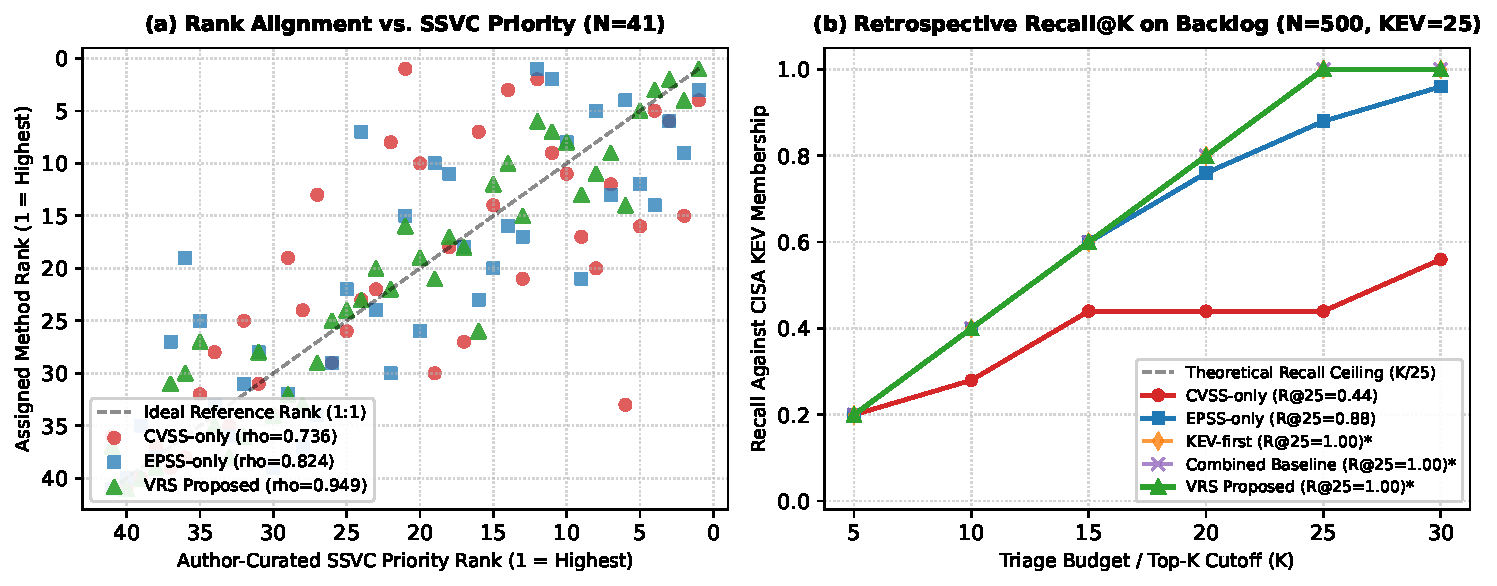
\includegraphics[width=\columnwidth]{../../experiments/results/figures/fig1.pdf}
\caption{Exploratory policy concordance on the 41-CVE benchmark (a) and 500-CVE KEV-concordance snapshot (b). These retrospective checks are separate from TEOB.}
\label{fig:ranking_and_recall}
\end{figure}

\begin{table}[t]
\centering
\caption{Exploratory 41-CVE SSVC-inspired benchmark (v1): baselines, context baselines, and ablations. Source: \texttt{experiments/results/metrics.json}, \texttt{statistics/}.}
\label{tab:exploratory}
\resizebox{\columnwidth}{!}{%
\begin{tabular}{lcccc}
\toprule
\textbf{Method / Variant} & \textbf{NDCG@10} & \textbf{P@10 (Act)} & \textbf{R@10 (Act)} & \textbf{Spearman $\rho$} \\
\midrule
CVSS-only               & 0.7563 & 0.6000 & 0.4000 & 0.7357 \\
EPSS-only               & 0.9217 & 0.8000 & 0.5333 & 0.8237 \\
KEV-first               & 0.7945 & 0.7000 & 0.4667 & 0.8247 \\
CVSS+EPSS+KEV           & 0.9513 & 0.9000 & 0.6000 & 0.8800 \\
EPSS$\times$Context     & 1.0000 & --     & 0.6667 & 0.9334 \\
VRS (No Context)        & 0.9513 & 0.9000 & 0.6000 & 0.8782 \\
\textbf{VRS (vrs-v1)}   & \textbf{1.0000} & \textbf{1.0000} & \textbf{0.6667} & \textbf{0.9488} \\
\bottomrule
\end{tabular}%
}
\end{table}

\subsection{Guardrail, Score Integrity, and Explanation Quality (RQ3)}
We evaluated the prototype keyword guardrail on a 60-case author-written corpus (Table~\ref{tab:guard}). Only the 48 retrieved-content cases are inspected; 12 query/banner/description cases are not inspected by \texttt{evidence\_validator}. On the 48 inspected cases, TPR is 0.36 $[0.20, 0.55]$, FPR is 0.30 $[0.16, 0.51]$, precision is 0.56, accuracy is 0.52, and F1 is 0.44. False positives stem from benign advisory wording (e.g., \emph{bypass}), while false negatives include paraphrased instructions, Unicode obfuscation, and uninspected channels.

\begin{table}[t]
\centering
\caption{Prototype keyword guardrail on 48 inspected retrieved-content cases. Source: \texttt{experiments/revision/guardrail/metrics.json}.}
\label{tab:guard}
\begin{tabular}{lcc}
\toprule
 & \textbf{Predicted block} & \textbf{Predicted allow} \\
\midrule
Actual attack (25) & TP = 9 & FN = 16 \\
Actual benign (23) & FP = 7 & TN = 16 \\
\bottomrule
\end{tabular}
\end{table}

In a 5-payload stub-LLM simulation through \texttt{chat\_with\_validation} (Table~\ref{tab:integrity}), the numeric \texttt{vrs\_score} was never corrupted (0/5 changes). However, the unmodified assistant allowed priority downgrades on KEV-listed findings (2/5 pass); adding the deterministic KEV priority floor raised this to 5/5. Non-KEV priority strings remain unconstrained by the Pydantic parser. \textbf{Explanation quality was not measured} (\texttt{explanation\_evaluation.csv} contains 0 rows), so no claim of explanation accuracy or analyst utility is made.

\begin{table}[t]
\centering
\caption{Score-integrity simulation (5 stub-LLM payloads). Source: \texttt{experiments/revision/guardrail/score\_integrity.json}.}
\label{tab:integrity}
\resizebox{\columnwidth}{!}{%
\begin{tabular}{lcc}
\toprule
\textbf{Payload} & \textbf{Unmodified} & \textbf{With KEV floor} \\
\midrule
S01: score 0, priority low (KEV) & fail (priority) & pass \\
S02: priority low (KEV)          & fail (priority) & pass \\
S03: priority high (non-KEV)     & pass            & pass \\
S04: retrieved doc requests low  & fail (priority) & pass \\
S05: unexpected priority field   & pass            & pass \\
\midrule
Total                            & 2 / 5           & 5 / 5 \\
\bottomrule
\end{tabular}%
}
\end{table}

\section{Discussion}
TEOB demonstrates that combining historical CVSS and EPSS signals improves ranking concordance with 90-day future CISA KEV additions compared with CVSS-only and EPSS-only on select metrics, while remaining statistically indistinguishable from equal-weight \texttt{CVSS+EPSS+KEV}. Crucially, because historical asset context is unavailable and pre-cutoff KEV entries are excluded, TEOB evaluates only $0.25C + 0.20E$ and does \textbf{not} validate VRS's KEV, exposure, or criticality weights. Conversely, the 41-CVE benchmark isolates context sensitivity ($-0.0706$ Spearman drop without context) but suffers from label circularity and ties with \texttt{EPSS$\times$Context}. Together, these findings support Vulture-AI's architectural separation of deterministic scoring from LLM prose, while showing that its prototype regex guardrail (TPR 0.36, FPR 0.30) is insufficient as a standalone injection defense.

\section{Threats to Validity and Limitations}
\begin{itemize}
    \item \textbf{KEV outcome proxy:} Future CISA KEV addition reflects federal-reported exploitation, not exhaustive real-world exploitation or organizational remediation urgency. Also, using a single \texttt{2026.10.13} snapshot cannot detect hypothetical additions later removed before \texttt{2026-10-13}.
    \item \textbf{Sparse positives and missing CVSS v4.0:} Only 11 of 7,927 CVEs (0.139\%) entered KEV within 90 days, producing wide bootstrap intervals. Additionally, 518 CVEs had CVSS v4.0 only and were treated as missing CVSS v3.x.
    \item \textbf{Exploratory benchmark limits:} The 41-CVE set is small, author-graded without inter-rater agreement, and shares inputs with VRS; weights remain exploratory and uncalibrated.
    \item \textbf{Unmeasured components:} Explanation quality (0 ratings), scanner-to-CVE matching accuracy, live frontier-LLM behavior, and SSVC tree comparison remain unmeasured.
\end{itemize}

\section{Conclusion}
Vulture-AI separates deterministic vulnerability scoring from retrieval-augmented LLM explanation. On the temporally separated 7,927-CVE TEOB cohort, VRS achieved higher point estimates than single-signal baselines (significant on Recall@50 vs CVSS-only and AP vs EPSS-only) but did not significantly outperform CVSS+EPSS+KEV, and effectively tested only a reduced CVSS+EPSS configuration. A deterministic KEV priority floor preserved score and KEV-priority integrity across 5 stub-LLM payloads, whereas the prototype keyword guardrail showed weak detection (TPR 0.36, FPR 0.30) and explanation quality remains unmeasured. Multi-month temporal cohorts, independent asset context, stronger prompt-injection defenses, and human explanation evaluations are needed before operational deployment claims can be made.

\enlargethispage{2\baselineskip}
\bibliographystyle{IEEEtran}
\bibliography{references_revised}

\end{document}
